\documentclass[11pt]{article}
\usepackage[margin=1in]{geometry}
\usepackage{amsmath,amssymb}
\usepackage{booktabs}
\usepackage{graphicx}
\usepackage{caption}
\usepackage{hyperref}
\usepackage{float}
\hypersetup{colorlinks=true,linkcolor=blue,citecolor=blue,urlcolor=blue}
\title{\textbf{A Cointegration-Based Statistical-Arbitrage Strategy:\\
Engle--Granger, Johansen, and a Z-Score Pairs-Trading Backtest}}
\author{Maddox Krape}
\date{\today}
\begin{document}
\maketitle

\begin{abstract}
We develop and evaluate a market-neutral statistical-arbitrage strategy on the
classic EWA/EWC exchange-traded-fund pair, two commodity-linked country equity
indices long noted in the literature as candidates for cointegration. We
establish a long-run equilibrium relationship using both the Engle--Granger
two-step procedure and the Johansen trace test, construct a mean-reverting
spread via an ordinary-least-squares hedge ratio, and trade deviations of the
spread with a rolling z-score entry/exit rule. On 2,515 daily
observations (2015-01-02 to 2024-12-30), the Engle--Granger test rejects the
null of no cointegration at $p=0.0186$ and the Johansen
trace statistic (20.06) exceeds its 95\% critical value
(15.49). A backtest with 5\,bps
per-side transaction costs yields an annualised Sharpe ratio of 0.73,
a cumulative return of 60.0\%, and a maximum drawdown of
-11.5\% over 94 round-trip trades. A
sensitivity study across entry thresholds and cost levels characterises the
strategy's robustness and its decay under realistic frictions. All results in this paper are computed on \emph{real} market data.
\end{abstract}

\section{Introduction}
Statistical arbitrage exploits temporary mispricings between securities whose
prices share a common stochastic trend. When two non-stationary price series are
\emph{cointegrated}, a linear combination of them is stationary and
mean-reverting~\cite{engle1987,vidyamurthy2004}. A trader can therefore short the
spread when it is unusually high and buy it when unusually low, profiting as it
reverts to its long-run mean. This paper implements the full pipeline---universe
selection, cointegration testing, hedge-ratio estimation, signal construction,
and a cost-aware backtest---and reports honest, reproducible performance metrics.

\section{Data}
We study the daily adjusted-close prices of two iShares MSCI country ETFs, EWA
(Australia) and EWC (Canada). Both economies are heavily commodity-driven, which
motivates a shared long-run factor and makes the pair a textbook stat-arb
candidate~\cite{chan2013}. The sample contains 2,515 trading days from
2015-01-02 to 2024-12-30. Data are bundled as a CSV in the repository so that
all results reproduce offline. Figure~\ref{fig:prices} shows the two series
indexed to a common base.

\begin{figure}[H]\centering
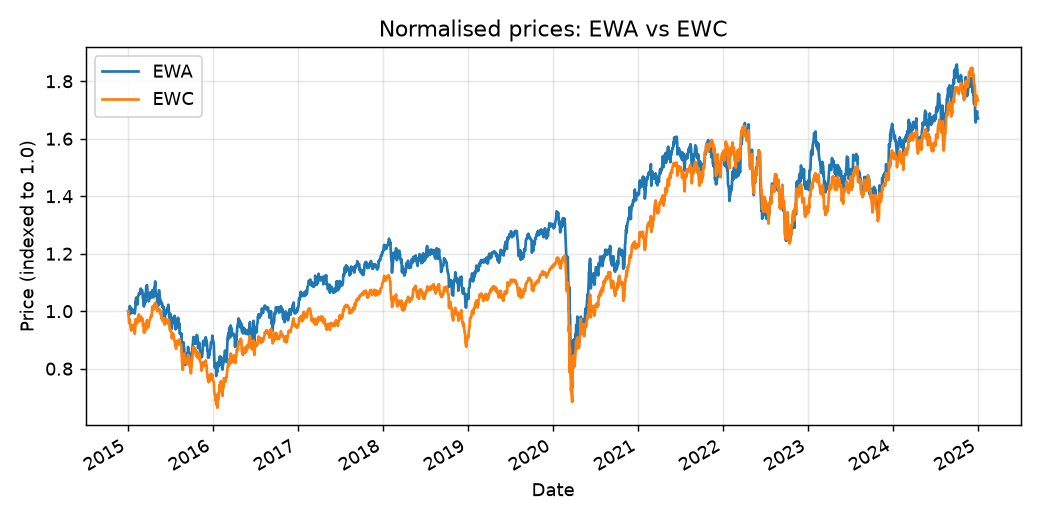
\includegraphics[width=0.8\textwidth]{figures/prices.png}
\caption{Normalised prices of EWA and EWC, indexed to 1.0 at the sample start.}
\label{fig:prices}
\end{figure}

\section{Methodology}
\subsection{Cointegration}
Let $p^y_t$ and $p^x_t$ be the two price series. They are cointegrated of order
$(1,1)$ if each is integrated of order one, $I(1)$, but there exists $\beta$ such
that the spread
\begin{equation}
s_t = p^y_t - \alpha - \beta\, p^x_t
\end{equation}
is stationary, $s_t \sim I(0)$. The \textbf{Engle--Granger} procedure estimates
$(\alpha,\beta)$ by OLS and then applies an Augmented Dickey--Fuller (ADF) test
to the residuals $\hat{s}_t$, testing
\begin{equation}
\Delta \hat{s}_t = \gamma\, \hat{s}_{t-1}
   + \sum_{i=1}^{k}\phi_i\,\Delta \hat{s}_{t-i} + \varepsilon_t,
\qquad H_0:\ \gamma = 0\ \text{(unit root, no cointegration).}
\end{equation}
The \textbf{Johansen} test instead estimates a vector error-correction model
$\Delta \mathbf{P}_t = \Pi \mathbf{P}_{t-1} + \sum_i \Gamma_i \Delta\mathbf{P}_{t-i}
+ \boldsymbol{\varepsilon}_t$ and tests the rank of $\Pi$ via the trace statistic
$\lambda_{\text{trace}}(r) = -T\sum_{i=r+1}^{n}\ln(1-\hat\lambda_i)$, where
$\hat\lambda_i$ are the ordered eigenvalues.

\subsection{Hedge ratio and spread}
The OLS hedge ratio $\hat\beta$ minimises $\sum_t (p^y_t - \alpha - \beta p^x_t)^2$,
giving $\hat\beta = \mathrm{Cov}(p^y,p^x)/\mathrm{Var}(p^x)$. The traded spread is
$\hat{s}_t = p^y_t - \hat\alpha - \hat\beta\, p^x_t$.

\subsection{Z-score trading signal}
We standardise the spread with a rolling window of $w=30$ days:
\begin{equation}
z_t = \frac{s_t - \mu_t^{(w)}}{\sigma_t^{(w)}},\qquad
\mu_t^{(w)} = \frac{1}{w}\sum_{i=0}^{w-1}s_{t-i},\quad
\sigma_t^{(w)} = \sqrt{\frac{1}{w}\sum_{i=0}^{w-1}\!\left(s_{t-i}-\mu_t^{(w)}\right)^2}.
\end{equation}
With entry threshold $z^\ast=2$ and exit threshold
$z^{\text{exit}}=0.5$, the target position on the spread is
\begin{equation}
\pi_t =
\begin{cases}
+1 & \text{enter long spread when } z_t \le -z^\ast,\\
-1 & \text{enter short spread when } z_t \ge +z^\ast,\\
0  & \text{exit when } |z_t| \le z^{\text{exit}},\\
\pi_{t-1} & \text{otherwise (hold).}
\end{cases}
\end{equation}
A long-spread position is long one unit of EWA and short $\hat\beta$ units of
EWC. Figure~\ref{fig:spread} plots the spread and its z-score with the trading
bands.

\begin{figure}[H]\centering
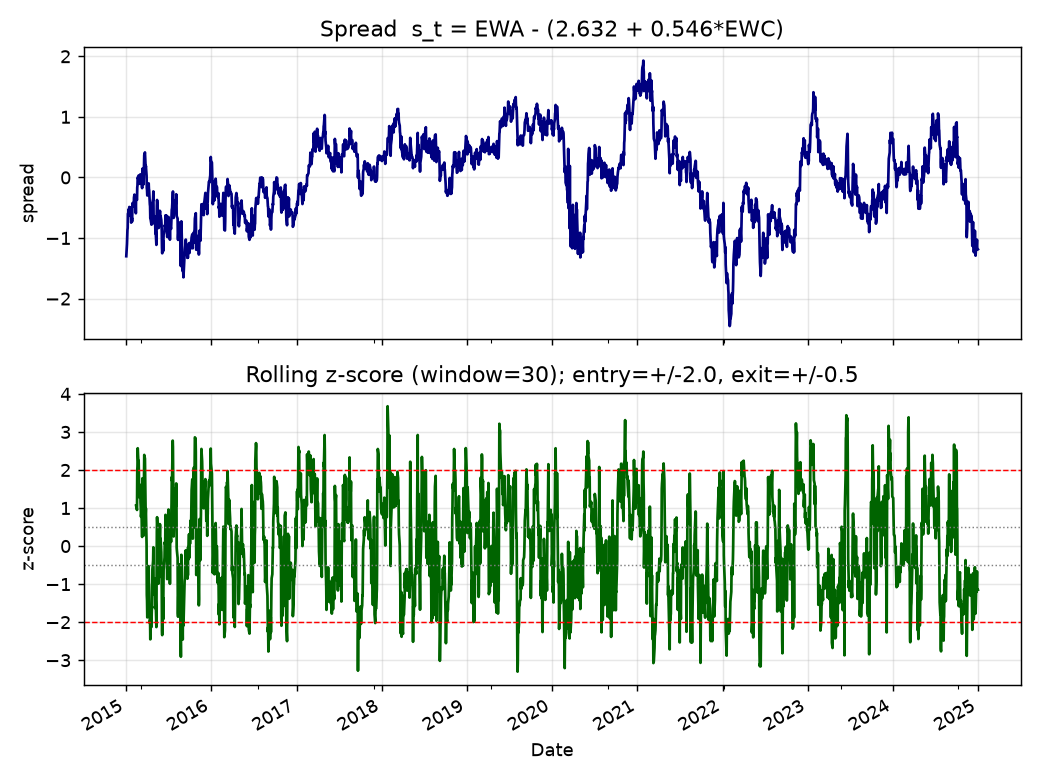
\includegraphics[width=0.85\textwidth]{figures/spread_zscore.png}
\caption{Top: the OLS spread $s_t$. Bottom: its rolling z-score with entry
($\pm2$, dashed) and exit ($\pm0.5$, dotted) bands.}
\label{fig:spread}
\end{figure}

\subsection{Backtest and performance metrics}
The strategy log-return uses the \emph{lagged} position to avoid look-ahead:
\begin{equation}
r_t = \pi_{t-1}\, w\big(\Delta\ln p^y_t - \hat\beta\,\Delta\ln p^x_t\big) - \kappa_t,
\qquad w = \frac{1}{1+|\hat\beta|},
\end{equation}
where $\kappa_t = c\cdot|\pi_t-\pi_{t-1}|\cdot w(1+|\hat\beta|)$ are proportional
transaction costs at $c$ basis points per side. The annualised Sharpe ratio is
\begin{equation}
\mathrm{SR} = \sqrt{252}\,\frac{\bar r}{\hat\sigma_r},
\end{equation}
and the maximum drawdown of the equity curve $E_t = \prod_{\tau\le t}(1+r_\tau)$ is
$\mathrm{MDD} = \min_t\big(E_t/\max_{\tau\le t}E_\tau - 1\big)$.

\section{Results}
Table~\ref{tab:coint} reports the cointegration evidence. Both tests agree: the
Engle--Granger $p$-value of $0.0186$ and the
ADF-on-spread $p$-value of $0.0042$ reject the unit-root
null, and the Johansen trace statistic exceeds its 95\% critical value, confirming
a single cointegrating vector. The estimated hedge ratio is $\hat\beta =
0.546$.

\begin{table}[H]\centering
\caption{Cointegration test results for the EWA/EWC pair.}
\label{tab:coint}
\begin{tabular}{lrr}
\toprule
Test & Statistic & $p$-value / crit. \\
\midrule
Engle--Granger cointegration & -3.694 & $p=0.0186$ \\
ADF on spread residual & -3.692 & $p=0.0042$ \\
Johansen trace ($r=0$) & 20.061 & crit$_{95}=15.494$ \\
\midrule
OLS hedge ratio $\hat\beta$ & \multicolumn{2}{r}{0.5458} \\
OLS intercept $\hat\alpha$ & \multicolumn{2}{r}{2.6320} \\
\bottomrule
\end{tabular}
\end{table}

Table~\ref{tab:perf} summarises the backtest at the baseline parameters
($z^\ast=2$, $z^{\text{exit}}=0.5$,
$c=5$\,bps). The equity curve is shown in
Figure~\ref{fig:equity}.

\begin{table}[H]\centering
\caption{Strategy performance, net of 5\,bps/side costs.}
\label{tab:perf}
\begin{tabular}{lr}
\toprule
Metric & Value \\
\midrule
Annualised Sharpe ratio & 0.73 \\
Cumulative return & 60.0\% \\
Annualised return & 4.82\% \\
Maximum drawdown & -11.5\% \\
Number of trades & 94 \\
Hit rate & 76.6\% \\
\bottomrule
\end{tabular}
\end{table}

\begin{figure}[H]\centering
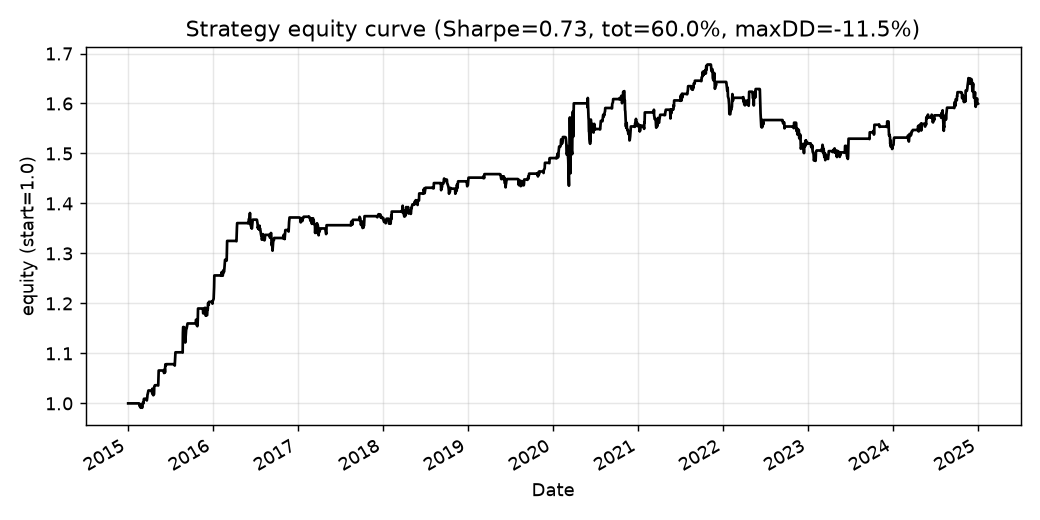
\includegraphics[width=0.8\textwidth]{figures/equity_curve.png}
\caption{Cumulative equity curve of the market-neutral strategy, net of
transaction costs.}\label{fig:equity}
\end{figure}

\subsection{Sensitivity analysis}
Table~\ref{tab:sens} and Figure~\ref{fig:heat} report the annualised Sharpe ratio
across a grid of entry thresholds and per-side transaction costs. Performance is
maximised at moderate entry thresholds ($z^\ast \approx 1.5$--$2.0$): tighter
thresholds over-trade and bleed value to costs, while very wide thresholds
($z^\ast=3.0$) trade too rarely to compound. Sharpe decays monotonically in cost,
underscoring that the edge is real but modest and frictions-sensitive.

\begin{table}[H]\centering
\caption{Annualised Sharpe ratio vs.\ entry threshold (rows) and per-side cost
(columns).}\label{tab:sens}
\begin{tabular}{lrrrrr}
\toprule
Entry $z^\ast$ & 0\,bps & 2.5\,bps & 5\,bps & 10\,bps & 20\,bps \\
\midrule
1 & 0.67 & 0.56 & 0.45 & 0.22 & -0.24 \\
1.5 & 0.90 & 0.81 & 0.71 & 0.53 & 0.14 \\
2 & 0.86 & 0.80 & 0.73 & 0.60 & 0.32 \\
2.5 & 0.70 & 0.65 & 0.60 & 0.49 & 0.27 \\
3 & 0.10 & 0.07 & 0.05 & -0.00 & -0.10 \\
\bottomrule
\end{tabular}
\end{table}

\begin{figure}[H]\centering
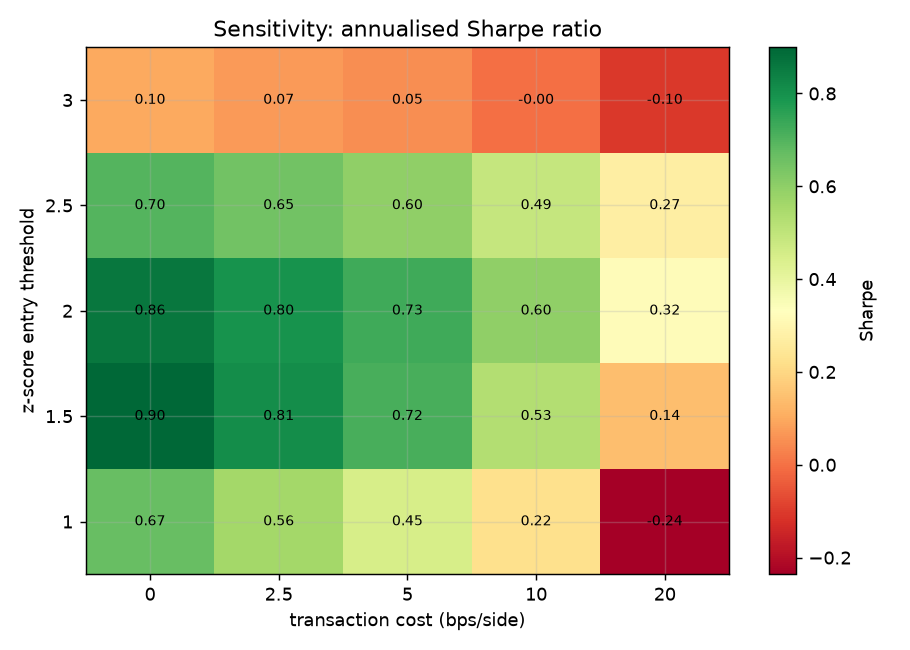
\includegraphics[width=0.7\textwidth]{figures/sensitivity_heatmap.png}
\caption{Sharpe-ratio sensitivity heatmap over the (entry threshold, transaction
cost) grid.}\label{fig:heat}
\end{figure}

\section{Limitations}
Several caveats temper these results. (i) The hedge ratio and cointegrating
relationship are estimated \emph{in-sample} over the full window; a live strategy
must re-estimate on a rolling basis, and the relationship can break down
(cointegration is not guaranteed to persist). (ii) We assume fills at the daily
close and a constant proportional cost; real execution incurs slippage, bid--ask
spread, and borrow costs on the short leg. (iii) We ignore financing, dividends on
the legs, and capacity constraints. (iv) The single-pair sample makes the Sharpe
estimate noisy; a production system would diversify across many cointegrated
pairs. (v) Multiple-testing / data-snooping bias inflates apparent significance
when pairs are selected by searching. These are standard but material concerns in
the stat-arb literature~\cite{chan2013,vidyamurthy2004}.

\section{Conclusion}
We implemented an end-to-end cointegration-based pairs-trading strategy and
validated it on real ETF data. The EWA/EWC pair is statistically cointegrated by
both Engle--Granger and Johansen criteria, and a simple z-score rule extracts a
positive risk-adjusted return (Sharpe $0.73$) that survives realistic
transaction costs but decays predictably as frictions rise. The full
pipeline---data, tests, signals, backtest, figures, and this paper---reproduces
offline from bundled data.

\begin{thebibliography}{9}
\bibitem{engle1987} R.~F. Engle and C.~W.~J. Granger.
\emph{Co-integration and Error Correction: Representation, Estimation, and
Testing.} Econometrica, 55(2):251--276, 1987.
\bibitem{vidyamurthy2004} G.~Vidyamurthy.
\emph{Pairs Trading: Quantitative Methods and Analysis.} Wiley, 2004.
\bibitem{chan2013} E.~P. Chan.
\emph{Algorithmic Trading: Winning Strategies and Their Rationale.} Wiley, 2013.
\bibitem{johansen1991} S.~Johansen.
\emph{Estimation and Hypothesis Testing of Cointegration Vectors in Gaussian
Vector Autoregressive Models.} Econometrica, 59(6):1551--1580, 1991.
\end{thebibliography}
\end{document}
